\chapter{Background}
In questo capitolo verrà descritta la tecnologia alla base di Bitcoin. Particolare attenzione verrà data alla blockchain, la struttura dati che costituisce il libro contabile, al funzionamento delle transazioni, agli indirizzi per introdurre infine la questione relativa all'anonimato. 
%1- Spiegare cosa sono i btcoin("storia" ecc...)
%2- Spiegare la blockchain(definizione)
%3- Spiegare address, wallet(anonimato), generazione indirizzi
%4- concentrarsi sulle transazioni(differenza teoria e pratica anonimato), come avvengono come funzionano %la fee ecc...
%Ricorda di mettere immagini
\section{Bitcoin}
Bitcoin, l’unità monetaria elettronica a cui facciamo riferimento in questa tesi, è stata sviluppata da Satoshi Nakamoto, un misterioso autore giapponese la cui identità resta a tutt'oggi ignota, tanto da indurre molti a pensare che si tratti di uno pseudonimo, o che dietro a tale nome si celi in realtà non una singola persona, ma addirittura un gruppo di ricercatori o di informatici. L’articolo in cui viene presentato l’intero protocollo Bitcoin viene pubblicato nel 2008, sotto il nome di ”Bitcoin: A Peer-to-Peer Electronic Cash System”\cite{nakamoto2009bitcoin}; il paper è facilmente reperibile e contiene la descrizione dettagliata del protocollo alla base del funzionamento di Bitcoin.\\La peculiarità di tale sistema è l’uso di una rete secondo il modello Peer-to-Peer per effettuare, diffondere e validare le transazioni, e l’intero storico di esse viene mantenuto in un libro contabile distribuito e di pubblica consultazione. La grande e difficile sfida che Bitcoin dunque si pone è quella di coniugare l’anonimato degli utenti con un’alta affidabilità relativamente alle transazioni e alla loro validità e integrità.\\A fronte della sfida di trasparenza versus affidabilità, è fondamentale definire un’implementazione del libro contabile che impedisca alterazioni di transazioni già registrate e validate: ricordiamo che in questo contesto paritario e distribuito, nessun controllo viene effettuato da parte di entità centrali, come per esempio le banche.\\
La soluzione ideata da Nakamoto per garantire l’integrità dello storico delle transazioni è stata quella di implementare il libro contabile tramite una particolare struttura dati: la blockchain.\\Come suggerisce il nome, la struttura si compone di una serie di blocchi collegati tra di loro come in una catena: ogni blocco racchiude un insieme di transazioni effettuate in un certo periodo temporale.\\Il blocco corrente, non ancora inserito, contiene le ultime transazioni la cui legittimazione deve essere ancora approvata, mentre i blocchi precedenti, già
agganciati alla catena, si riferiscono a transazioni già validate, e la blockchain è fin lì immutabile. Il meccanismo che garantisce la totale immutabilità della struttura, pena la sua completa invalidazione, è la crittografia.\\\\
\begin{figure}[h!]
    \centering
    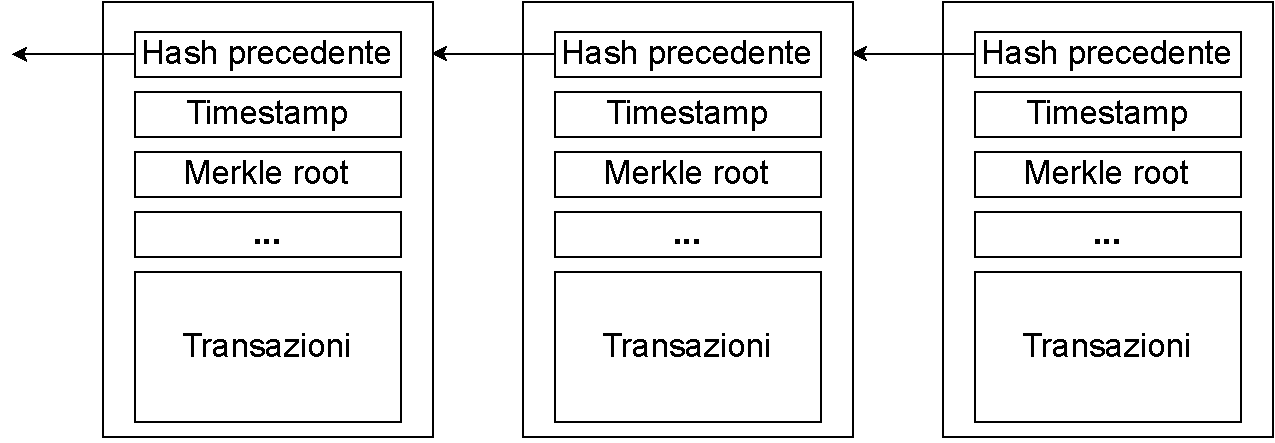
\includegraphics[scale=0.6]{Images/blockChaining.pdf}
    \caption{Schema della Blockchain}
    \label{fig:blockchain}
\end{figure}
\FloatBarrier
\section{Blockchain}

